\documentclass[12pt,a4paper]{report}

\usepackage[utf8]{inputenc}
\usepackage[spanish]{babel}
\usepackage{graphicx}
\usepackage{amsmath}
\usepackage{amssymb}
\usepackage{hyperref}
\usepackage{comment}
\usepackage{geometry}
\usepackage{caption}
\usepackage{subcaption}
\geometry{a4paper, margin=1in}

\title{Segmentación Multimodal para detección de Animales}
\author{
    Jorge Urbón Burgos \\
    \texttt{777295@unizar.es}
    \and
    Supervisor: Rosario Aragües \\
    \texttt{raragues@unizar.es}
    \and
    Co-Supervisor: Jesús Bermúdez \\
    \texttt{bermudez@unizar.es}
}
\date{\today}

\begin{document}

\maketitle

\begin{abstract}
% TODO: add abstract
\end{abstract}

\tableofcontents

\chapter{Introduction}
\label{chap:introduction}
Image segmentation has been a fundamental problem in computer vision tasks since the early days of the field. The main goal of image segmentation is to partition an image into multiple regions or objects

\chapter{Literature Review}
\label{chap:literature_review}
% TODO: add literature review

\chapter{Metodología}
\label{chap:methodology}
\section{Datos}
\label{sec:data}
\subsection{Lindenthal Dataset}
\label{subsec:lindenthal_dataset}
Para este trabajo, emplearemos una parte\footnote{A pesar de que este \textit{dataset} cuenta con 775 secuencias de video que incluyen información \texttt{RGB} durante el día o \texttt{IR} durante la noche, así como mapas de profundidad en ambos casos, tan solo fueron etiquetados para su uso como \textit{Ground Truth} 12 videos nocturnos, de los cuales se etiqueraría cada décimo fotograma.} del \textit{dataset} \texttt{Lindenthal Camera Traps} obtenido por \cite{haucke2021exploitingdepthinformationwildlife}. Este \textit{dataset} consiste en imágenes de animales en un entorno natural, obtenidas con una cámara estéreo \texttt{Intel RealSense D435} y en el que se incluyen imágenes infrarojas (\texttt{IR}) con una profundidad de 8 bits y mapas de profundidad (\texttt{D}) con una profundidad de 16 bits en los que el valor de cada pixel representa la distancia en milimetros\footnote{El sensor \texttt{Intel RealSense D435} cuenta con la capacidad de obtener imágenes estéreo de forma activa empleando ambas cámaras infrarojas mediante la proyección de un patrón infrarojo en la escena, sin embargo al haberse construido este dataset a partir de imagenes nocturnas en las que dicho patrón sería visible al sensor \texttt{IR}, se optó por generar los mapas de profundidad \texttt{D} mediante el uso de la cámara estéreo en modo pasivo.}. Ambas modalidades se encuentran ya alineadas y sincronizadas, lo que permite un fácil acceso a la información de ambas modalidades. Además, el etiquetado de los animales se encuentra en formato \texttt{COCO}. En la figura \ref{fig:base-data-lindenthal} se muestra un ejemplo de una pareja de imágenes \texttt{IR} y \texttt{D} del \textit{dataset}.
\begin{figure}
    \centering
    \begin{subfigure}{0.45\textwidth}
        \centering
        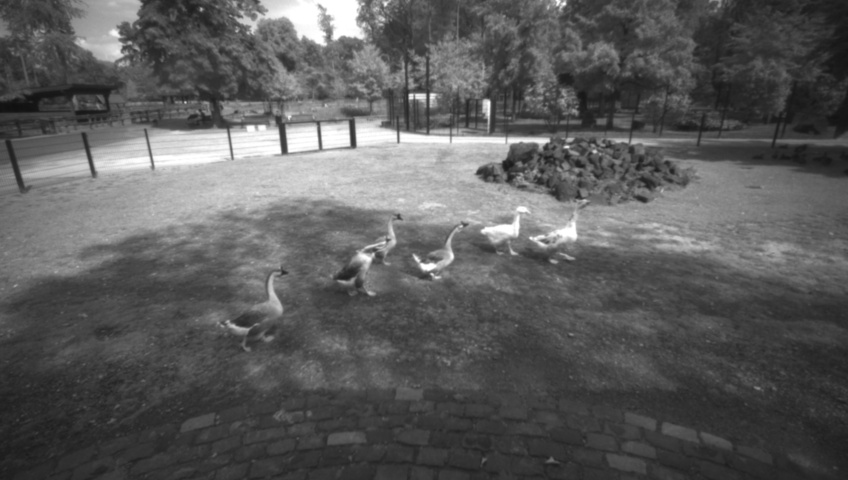
\includegraphics[width=\textwidth]{media/data/ir_gueese.jpg}
        \caption{Imagen \texttt{IR}}
    \end{subfigure}
    \hfill
    \begin{subfigure}{0.45\textwidth}
        \centering
        
\includegraphics[width=\textwidth]{media/data/depth_gueese.png}
        \caption{Imagen de profundidad}
    \end{subfigure}
    \caption{Ejemplo de una pareja \texttt{IR}-\texttt{D} del \textit{dataset} \texttt{Lindenthal Camera Traps}}
    \label{fig:base-data-lindenthal}
\end{figure}

\subsubsection{Desglose del \textit{Dataset}}
El dataset consiste en doce videos para los que se ha etiquetado cada décimo fotograma, lo que supone un total de 412 pares \texttt{IR}-\texttt{D} con 1038 instancias etiquetadas en formato \texttt{COCO} que incluyen la máscara, la caja delimitadora de la misma, la categoría y un identificador único para el animal. Las categorías de animales presentes en el dataset son \textbf{Deer}, \textbf{Goat}, \textbf{Donkey} y \textbf{Goose} y en la figura \ref{fig:dataset-breakdown} se muestra un desglose de la frecuencia de aparición de cada categoría en el dataset.
\begin{figure}
    \centering
    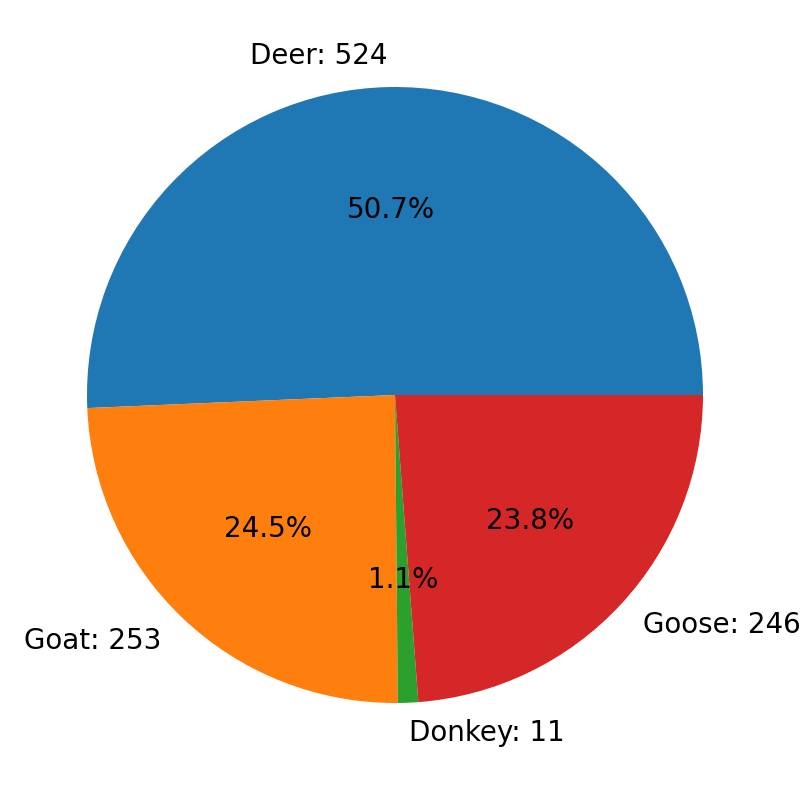
\includegraphics[width=0.5\textwidth]{media/data/dataset_breakdown.png}
    \caption{Desglose de la frecuencia de aparición de cada categoría en el dataset}
    \label{fig:dataset-breakdown}
\end{figure}
Por otra parte, este \textit{dataset} se dividirá en dos partes: el 85\% para entrenamiento y el 15\% restante para validación. En la figura \ref{fig:tagged-example} se muestra un ejemplo de un par \texttt{IR}-\texttt{D} con sus respectivas máscaras de segmentación.
\begin{figure}
    \centering
    \begin{subfigure}{0.45\textwidth}
        \centering
        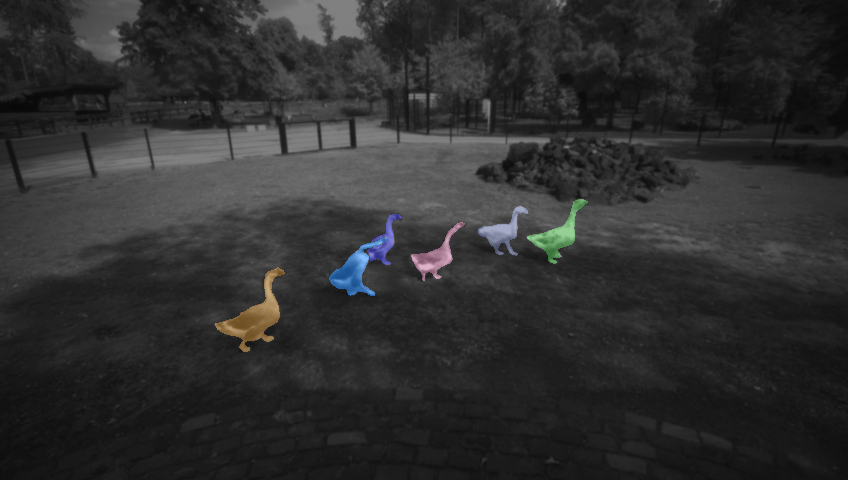
\includegraphics[width=\textwidth]{media/data/mask_gueese_ir.png}
        \caption{Imagen \texttt{IR} etiquetada}
    \end{subfigure}
    \hfill
    \begin{subfigure}{0.45\textwidth}
        \centering
        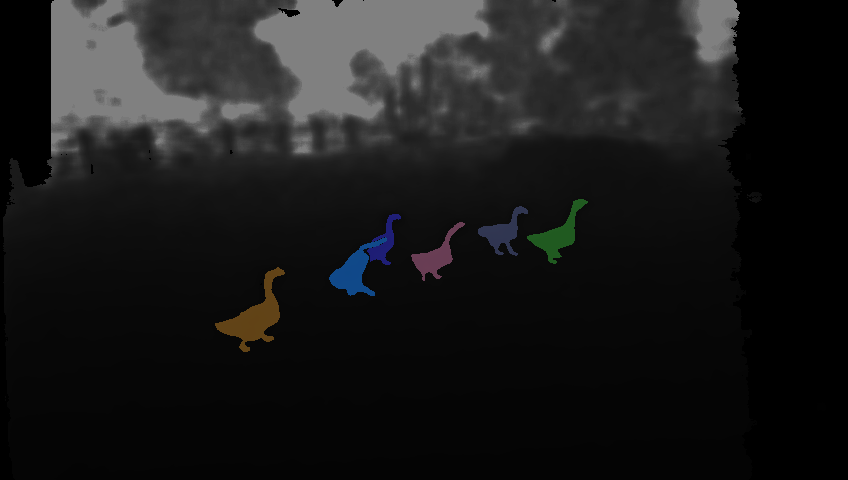
\includegraphics[width=\textwidth]{media/data/mask_gueese_de.png}
        \caption{Imagen de profundidad}
    \end{subfigure}
    \caption{Ejemplo de una pareja \texttt{IR}-\texttt{D} del \textit{dataset} \texttt{Lindenthal Camera Traps}}
    \label{fig:tagged-example}
\end{figure}

\section{Modelo}
\label{sec:model}
El modelo a implementar fue presentado por \cite{zhang2023cmxcrossmodalfusionrgbx} y propone una arquitectura de fusión de características de forma "interactiva" implementando rectificación de características inter-modal y bidireccional, así como atención cruzada secuencia a secuencia, lo que permite interacciones inter-modales más ricas y efectivas. La arquitectura propuesta por \cite{zhang2023cmxcrossmodalfusionrgbx} se muestra en la figura \ref{fig:cmx-architecture}.
\begin{figure}
    \centering
    \includegraphics[width=\textwidth]{media/model/cmx_architecture.png}
    \caption{Arquitectura propuesta por \cite{zhang2023cmxcrossmodalfusionrgbx}}
    \label{fig:cmx-architecture}
\end{figure}

\subsection{Entrenamiento}
\label{subsec:training}
Para entrenar el modelo, se empleará un \textit{backbone} pre-rentrenado en \texttt{ImageNet} y se empleará la técnica de \textit{transfer learning} para adaptar el modelo a las características de los datos de entrada. Se empleará la función de pérdida \texttt{CrossEntropyLoss} y el optimizador \texttt{Adam} con una tasa de aprendizaje de $10^{-6}$ dinámica. El modelo se entrenará durante 500 épocas con un tamaño de \textit{batch} de 2. Además, para fomentar el aprendizaje de las características inter-modales, se aplicará \textit{modality dropout} con una probabilidad de 0.5 decreciente con el número de épocas. Por último, se analizan las diferentes propuestas en \ref{subsec:tecnicas_post_procesado} con el fin de determinar qué técnica de pre-procesado es la más adecuada para el modelo.


\subsection{Técnicas de Pre-Procesado}
\label{subsec:tecnicas_post_procesado}
Cuando vamos a usar una imagen como input para un modelo de segmentación, se debe tener en cuenta el formato en el que se desea representar la información que se le proporciona al modelo. En este caso, se cuenta con dos modalidades de entrada: \texttt{IR} y \texttt{D}, por lo que se deben considerar las distintas técnicas de preprocesado que se pueden aplicar a cada modalidad para obtener un mejor resultado en la segmentación.
Existe una variedad de técnicas de pre-procesado que aprovechan los tres canales de entrada del modelo para así lograr un \textit{input} capaz de aportar mayor cantidad de información al modelo de segmentación. Además, al consistir el \textit{dataset} en imágenes obtenidas con una cámara estéreo \texttt{Intel RealSense D435}, la cantidad de ruido en las imágenes es considerable, por lo que toda técnica que ayude a destacar los objetos de interés será importante para el correcto desempeño del modelo. En este caso, debido a que la imagen \texttt{IR} ya cuenta con una calidad aceptable, se optará por aplicar las técnicas de pre-procesado exclusivamente a la imagen de profundidad \texttt{D}.

\begin{comment}

\subsubsection{Equalización del Histograma}
La primera técnica de postprocesado a implementar consiste en la equalización del histograma de valores en la imagen. Esto puede suponer una gran mejora en la forma en la que se representan las imágenes debido a que no todo el rango de valores de intensidad es aprovechado dado a que la mayoría de los objetos de interés se encuentran a una distancia relativamente baja de la cámara. Equalizar el histograma puede permitir destacar ciertos objetos que de otra forma no serían tan visibles.
\begin{figure}
    \centering
    \begin{subfigure}{0.45\textwidth}
        \centering
        
\includegraphics[width=\textwidth]{media/data/depth_gueese.png}
        \caption{Imagen de profundidad base}
    \end{subfigure}
    \hfill
    \begin{subfigure}{0.45\textwidth}
        \centering
        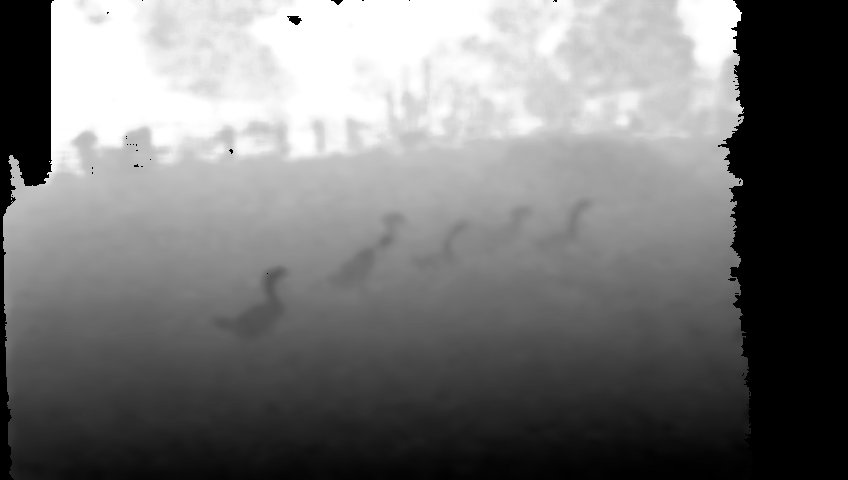
\includegraphics[width=\textwidth]{media/data/deptheq_gueese.png}
        \caption{Histograma equalizado}
    \end{subfigure}
    \caption{Comparación entre la imagen de profundidad base y la imagen con el histograma equalizado}
    \label{fig:depth-histeq-comparison}
\end{figure}
Como se puede observar en la figura \ref{fig:histogram-comparison}, la ecualización del histograma permite un mayor reparto de los valores de intensidad en la imagen, lo que aprovecha aquellos rangos menos utilizados en la imagen original permitiendo así un mayor contraste entre los rangos más utilizados en la imagen original como se puede observar en la figura \ref{fig:depth-histeq-comparison}.
Esta técnica, sin embargo, puede no ser adecuada para otras aplicaciones, ya que se pierde la información real sobre la distancia de los objetos a la cámara.
\begin{figure}
    \centering
    \begin{subfigure}{0.45\textwidth}
        \centering
        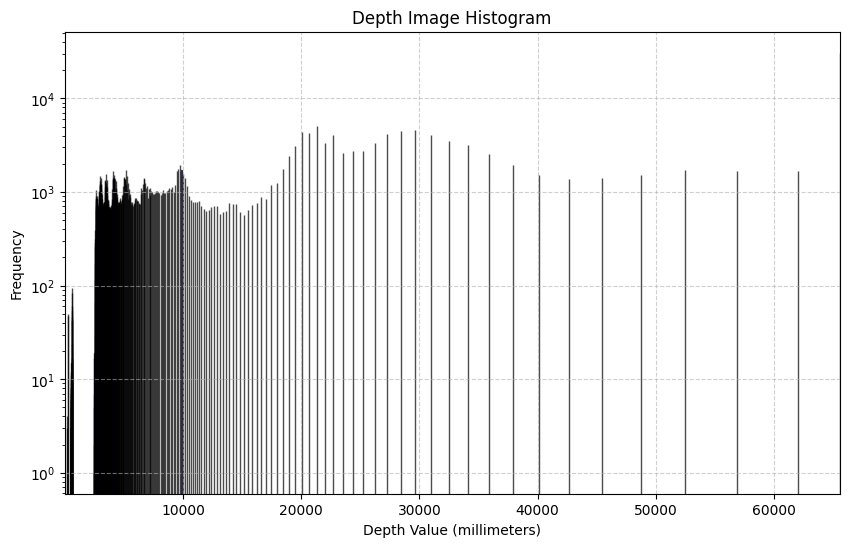
\includegraphics[width=\textwidth]{media/data/normal_histogram.png}
        \caption{Histograma de la imagen de profundidad base}
    \end{subfigure}
    \hfill
    \begin{subfigure}{0.45\textwidth}
        \centering
        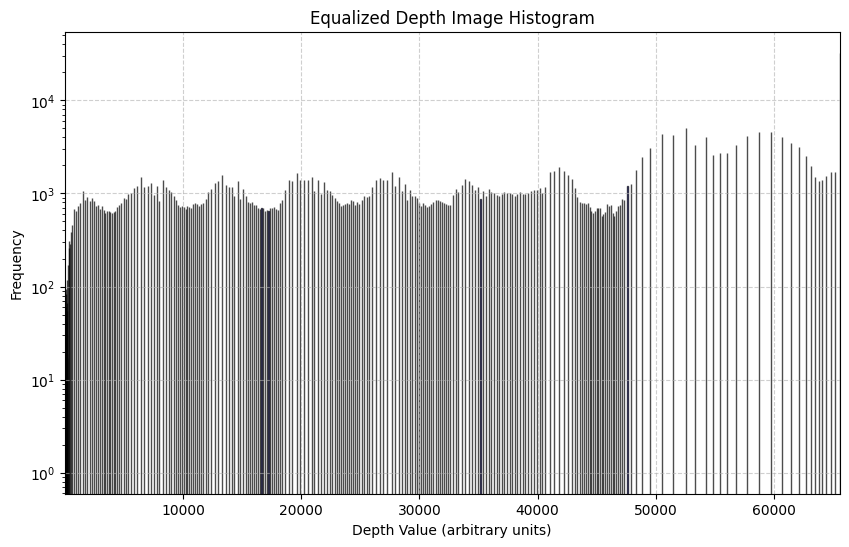
\includegraphics[width=\textwidth]{media/data/equalized_histogram.png}
        \caption{Histograma de la imagen con el histograma equalizado}
    \end{subfigure}
    \caption{Comparación entre los histogramas de la imagen de profundidad base y la imagen con el histograma equalizado}
    \label{fig:histogram-comparison}
\end{figure}
\end{comment}

\subsubsection{HHA Encoding}
\label{subsubsec:hha_encoding}
Esta técnica, propuesta por \cite{gupta2014learningrichfeaturesrgbd} usa los tres canales de la imagen de entrada para codificar las siguientes tres características:
\begin{itemize}
    \item Altura sobre el suelo
    \item Disparidad horizontal
    \item Ángulo con respecto a la gravedad
\end{itemize}
Estas colorización, además de implementar características que difícilmente serían aprendidas por el modelo si no se codificaran en la imagen de entrada, aprovecha los tres canales de entrada al \textit{encoder}, por lo que los pesos ya preentrenados en \textit{ImageNet} pueden ser empleados para una mejor comprensión de la escena.
\begin{figure}
    \centering
    \begin{subfigure}{0.45\textwidth}
        \centering
        
\includegraphics[width=\textwidth]{media/data/depth_gueese.png}
        \caption{Imagen de profundidad base}
    \end{subfigure}
    \hfill
    \begin{subfigure}{0.45\textwidth}
        \centering
        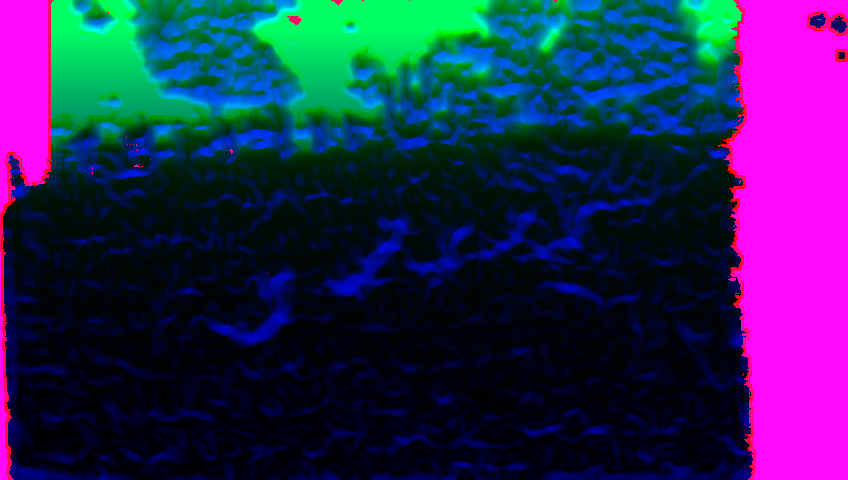
\includegraphics[width=\textwidth]{media/data/hha_gueese.png}
        \caption{Profundidad colorizada con HHA}
    \end{subfigure}
    \caption{Comparison between the base depth image and the HHA encoded image}
    \label{fig:depth-hha-comparison}
\end{figure}

\subsubsection{Colorizacón Jet}
\label{subsubsec:jet_colorization}
Como se propone en \cite{eitel2015multimodaldeeplearningrobust}, otra posible técnica es la colorización de la imagen de entrada usando el esquema de color \textit{Jet}, lo que implica la asignación de un valor \textit{RGB} a cada píxel dependiendo de su valor de intensidad. Esto, de forma similar a \ref{subsubsec:hha_encoding}, permite al modelo aprovechar sus pesos ya entrenados en \textit{ImageNet} para identificar con mayor facilidad los objetos a segmentar.
\begin{figure}
    \centering
    \begin{subfigure}{0.45\textwidth}
        \centering
        
\includegraphics[width=\textwidth]{media/data/depth_gueese.png}
        \caption{Imagen de profundidad base}
    \end{subfigure}
    \hfill
    \begin{subfigure}{0.45\textwidth}
        \centering
        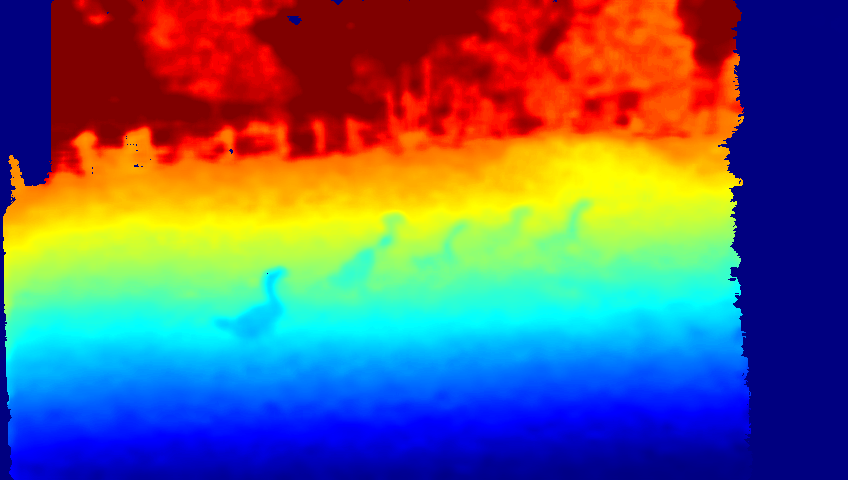
\includegraphics[width=\textwidth]{media/data/jet_gueese.png}
        \caption{Profundidad colorizada con \textit{Jet}}
    \end{subfigure}
    \caption{Comparación entre la imagen de profundidad y la colorización \textit{Jet}}
    \label{fig:depth-jet-comparison}
\end{figure}

\subsubsection{Colorización por Distancia}
Considerando los resultados obtenidos por Jet, se propone en una técnica de colorización que, si bien puede no resultar visualmente atractiva para el ojo humano, podría codificar la distancia de forma más efectiva para el modelo. Esta técnica también se basa en asignar un valor \texttt{RGB} a cada píxel dependiendo de su valor de intensidad, pero en este caso se determinará que los objetos más lejanos serán más dominados por el canal \texttt{R}, mientras que los objetos más cercanos serán más dominados por el canal \texttt{B} pasando por el canal \texttt{G} en el rango intermedio. La interpolación de los valores de distancia a estos valores podría permitir al modelo aprender de forma más efectiva la distancia de los objetos en la escena y así poder segmentarlos de forma más efectiva.

\subsubsection{Normales}
\label{subsubsec:normals}
Siguiendo lo propuesto por \cite{eitel2015multimodaldeeplearningrobust}, una mejor y más rápida solución de postprocesado consiste en la codificación de las normales en la imagen de entrada. Esta técnica consiste en calcular el vector normal de la superficie de cada pixel partiendo de la imagen de profundidad y codificarlo en los tres canales del \textit{input} del modelo. Esto permite al modelo aprender características de la escena que de otra forma serían difíciles de aprender, como la orientación de los objetos en la escena.
\begin{figure}
    \centering
    \begin{subfigure}{0.45\textwidth}
        \centering
        
\includegraphics[width=\textwidth]{media/data/depth_gueese.png}
        \caption{Imagen de profundidad base}
    \end{subfigure}
    \hfill
    \begin{subfigure}{0.45\textwidth}
        \centering
        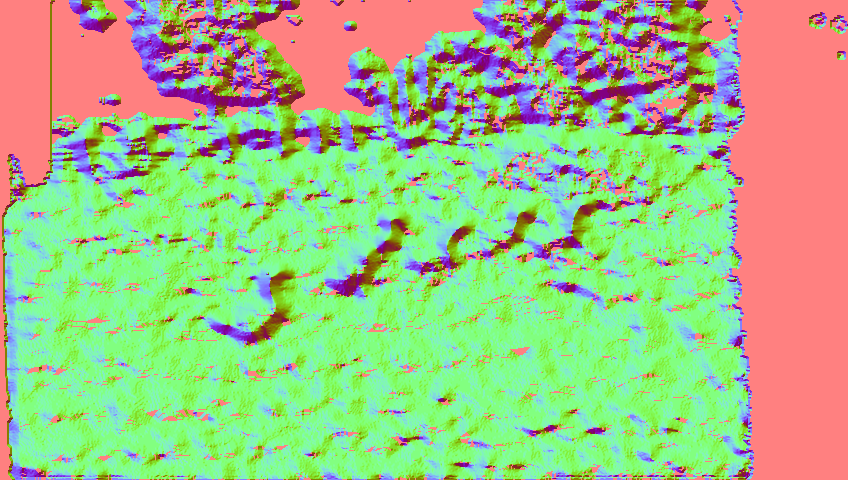
\includegraphics[width=\textwidth]{media/data/normal_gueese.png}
        \caption{Normales codificadas en la imagen de profundidad}
    \end{subfigure}
    \caption{Comparación entre la imagen de profundidad y la codificación de las normales}
    \label{fig:depth-normals-comparison}
\end{figure}

\subsubsection{Comparación de Técnicas}
\label{subsubsec:techniques_comparison}
Las distintas técnicas anteriores presentan diferentes resultados a la hora de ser aplicadas al \textit{input} del modelo. La tabla \ref{tab:techniques-comparison} muestra una comparación entre las distintas técnicas de postprocesado.
\begin{table}
    \centering
    \begin{tabular}{|c|c|c|c|c|c|}
        \hline
        Técnica & Depth & HHA & Jet & Normales & Distance \\
        \hline
        \hline
        Background IoU & 99.831 & 99.807 & 99.808 & 99.807 & 99.810 \\
        \hline
        Deer IoU & 81.790 & 78.884 & 78.872 & 79.353 & 78.987\\
        \hline
        Goat IoU & 78.947 & 79.282 & 80.102 & 74.442 & 79.442\\
        \hline
        Donkey IoU & 74.109 & 75.623 & 76.267 & 76.166 & 74.541 \\
        \hline
        Goose IoU & 78.009 & 76.111 & 75.988 & 76.486 & 76.544\\
        \hline
        \textbf{Mean} IoU & 82.537 & 81.941 & 82.208 & 81.251 & 81.865\\
        \hline
    \end{tabular}
    \caption{Evaluación \texttt{IR}-\texttt{D} entre las distintas técnicas de postprocesado}
    \label{tab:techniques-ird-comparison}
\end{table}
\begin{table}
    \centering
    \begin{tabular}{|c|c|c|c|c|c|}
        \hline
        Técnica & Depth & HHA & Jet & Normales & Distance \\
        \hline
        \hline
        Background IoU & 99.823 & 99.801 & 99.795 & 99.799 & 99.800\\
        \hline
        Deer IoU & 81.361 & 78.797 & 78.063 & 78.830 & 78.457\\
        \hline
        Goat IoU & 78.010 & 79.187 & 78.596 & 77.266 & 79.026\\
        \hline
        Donkey IoU & 71.146 & 67.713 & 75.221 & 63.912 & 73.968\\
        \hline
        Goose IoU & 76.326 & 74.934 & 73.149 & 74.297 & 74.089\\
        \hline
        \textbf{Mean} IoU & 81.333 & 78.513 & 80.965 & 78.821 & 81.068\\
        \hline
    \end{tabular}
    \caption{Evaluación \texttt{IR} entre las distintas técnicas de postprocesado}
    \label{tab:techniques-ir-comparison}
\end{table}
\begin{table}
    \centering
    \begin{tabular}{|c|c|c|c|c|c|}
        \hline
        Técnica & Depth & HHA & Jet & Normales & Distance\\
        \hline
        \hline
        Background IoU & 99.598 & 99.530 & 99.561 & 99.552 & 99.568\\
        \hline
        Deer IoU & 52.348 & 43.681 & 46.818 & 45.351 & 47.319\\
        \hline
        Goat IoU & 70.057 & 62.111 & 67.850 & 62.962 & 67.403\\
        \hline
        Donkey IoU & 65.208 & 64.397 & 64.213 & 72.583 & 71.497\\
        \hline
        Goose IoU & 56.162 & 49.537 & 54.352 & 52.797 & 54.595\\
        \hline
        \textbf{Mean} IoU & 68.675 & 63.851 & 66.559 & 66.649 & 68.077\\
        \hline
    \end{tabular}
    \caption{Evaluación \texttt{D} entre las distintas técnicas de postprocesado}
    \label{tab:techniques-d-comparison}
\end{table}

\chapter{Results}
\label{chap:results}
% TODO: add results

\chapter{Discussion}
\label{chap:discussion}
% TODO: add discussion

\chapter{Conclusion}
\label{chap:conclusion}
% TODO: add conclusion and future work

\bibliography{refs.bib}
\bibliographystyle{IEEEtran}

\appendix
\label{app:appendix_a}
% TODO: whatever appendices :)

\end{document}